\documentclass[11pt]{article}
\usepackage[margin=2.3cm]{geometry}
\usepackage[T1]{fontenc}
\usepackage{lmodern}
\usepackage{microtype}
\usepackage{booktabs}
\usepackage{array}
\usepackage{tabularx}
\usepackage{graphicx}
\usepackage{float}
\usepackage{needspace}
\usepackage{amsmath}
\usepackage{xcolor}
\usepackage[hidelinks]{hyperref}
\usepackage{enumitem}
\usepackage{caption}
\captionsetup{font=small,labelfont=bf}
\setlist{itemsep=2pt,topsep=3pt}
\newcolumntype{L}[1]{>{\raggedright\arraybackslash}p{#1}}
\newcolumntype{Y}{>{\raggedright\arraybackslash}X}
\newcommand{\code}[1]{\texttt{#1}}
\newcommand{\busy}{$^\dagger$}
\widowpenalty=10000
\clubpenalty=10000
\let\oldsection\section
\renewcommand{\section}{\Needspace{8\baselineskip}\oldsection}
\let\oldsubsection\subsection
\renewcommand{\subsection}{\Needspace{7\baselineskip}\oldsubsection}

\title{Why \code{mplcp} is fast, and why recent surveys do not feature it}
\author{RPOPT notes}
\date{14 November 2026}

\begin{document}
\maketitle

\section{Summary}

\code{mplcp} is RPOPT's implementation of the parametric linear complementarity (pLCP) pivoting method of Jones and
Morari \cite{jm2006}. On RPOPT's 12 MPC benchmark problems it is the fastest serial exact solver on 11 (on
masses2\_N4, \code{graph} is 1.2x faster). It is 1.2x to 1.8x faster than RPOPT's tuned \code{geometric}, 1.2x to
17x faster than RPOPT's port of the Arnstr\"om-Axehill algorithm, and 7x to over 60,000x faster than the pLCP
enumeration method of Herceg et al.\ \cite{herceg2015}. The reasons, in order of weight:

\begin{enumerate}
  \item \textbf{Neighbours are found algebraically.} The region across a facet is the basis reached by one pivot of
  the current tableau. There is no step over the facet, no LP or QP at a stepped point, and no set of candidate
  active sets to test.
  \item \textbf{One candidate per facet.} The pivot names exactly one neighbour. A neighbour already known is
  discarded by a hash lookup, not after an LP and a QP.
  \item \textbf{The region comes straight from the tableau.} Its law and inequalities are rows of the basis, and
  RPOPT settles their redundancy by bounding-box clipping. \code{mplcp} needs 1.6 to 5 LPs per region, against 23
  to 35 for \code{geometric} and 54 to 368 for the graph family.
  \item \textbf{Careful implementation.} A compact incremental tableau, one-pass child tableaux and a private region
  builder bring the cost down to about 10 to 30 \textmu s per region.
\end{enumerate}

\noindent The method is not unknown. It is the default solver of MPT3 \cite{mpt3}, a toolbox cited by over 1,300
papers. It is missing from recent surveys for five reasons:
\begin{itemize}
  \item the 2006 paper has no benchmarks, and claims only parity with other methods;
  \item users cite the toolbox, not the algorithm;
  \item benchmarks see it only through a MATLAB toolbox;
  \item the pLCP line is remembered by its slow enumeration variant;
  \item surveys follow their authors' own toolboxes.
\end{itemize}

\section{What \code{mplcp} does}

The KKT conditions of a strictly convex mpQP form a pLCP $w - Mz = q + R\theta$, $w, z \ge 0$, $w^\top z = 0$, with
$z$ the multipliers and $w$ the slacks. A critical region is a complementary basis $B$. In the tableau
$x_B = \rho(\theta) + T y_N$, the region is $\{\theta : \rho(\theta) \ge 0\}$, and the basic part of the tableau
gives the multipliers and the control law as affine functions of $\theta$. Starting from one basis, the method visits
its facets. Across each facet, the neighbouring basis is the one obtained by a principal pivot on the row that
becomes zero there. A lexicographic perturbation of $q$ makes every pivot unique, so each parameter belongs to
exactly one region and adjacency is exact even at degenerate vertices \cite{jm2006,columbano2009}.

\needspace{10\baselineskip}
Table~\ref{tab:families} contrasts how the main families find the next region.

\begin{table}[H]
\centering\small
\caption{How each family finds the next critical region.}
\label{tab:families}
\begin{tabularx}{\textwidth}{@{}L{5.4cm} Y@{}}
\toprule
family & step to the next region \\
\midrule
geometric \cite{tondel2003,spjotvold2006} & an LP for a facet centre, a step across the facet, a QP at the stepped point, then a region build; degenerate facets need extra work \\
combinatorial \cite{gupta2011} & enumerate candidate active sets, with a feasibility LP, a rank test and a multiplier test for each \\
graph and combinatorial graph & test candidate active sets adjacent to known regions, as above \\
pLCP enumeration \cite{herceg2015} & enumerate complementary bases row by row in a tree, with LP pruning \\
pLCP pivoting \cite{jm2006} (\code{mplcp}) & one principal pivot of the current tableau per facet \\
\bottomrule
\end{tabularx}
\end{table}

\section{Why it is fast}

\subsection{Measured speed}

\needspace{6\baselineskip}
Figure~\ref{fig:times} shows the single-thread solve time of RPOPT's exact solvers on five MPC problems. All solvers
return the same regions. The data come from an idle machine, as the faster median of two full runs.

\begin{figure}[H]
\centering
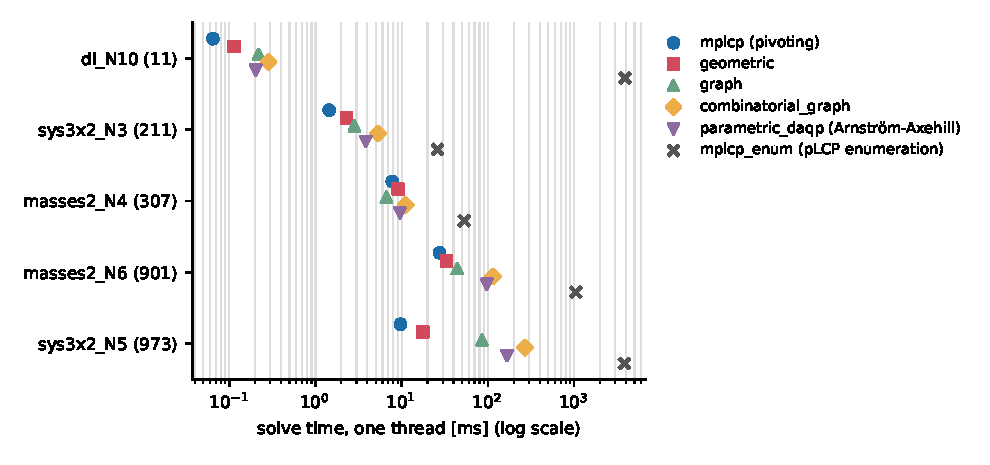
\includegraphics[width=\textwidth]{fig_times.pdf}
\caption{Single-thread solve time per problem (regions in parentheses). Source: \code{bench/results/rust.json}.}
\label{fig:times}
\end{figure}

\needspace{12\baselineskip}
\begin{table}[H]
\centering\small
\caption{Solve time in ms, one thread, with the ratio to \code{mplcp} in parentheses.}
\label{tab:times}
\setlength{\tabcolsep}{4.5pt}
\begin{tabular}{@{}lrrrrrr@{}}
\toprule
problem (regions) & \code{mplcp} & \code{geometric} & \code{graph} & \code{comb.\ graph} & \code{param.\ daqp} & \code{mplcp\_enum} \\
\midrule
di\_N10 (11) & 0.065 & 0.113 (1.7x) & 0.218 (3.4x) & 0.286 (4.4x) & 0.203 (3.1x) & 3,906 (60,242x) \\
sys3x2\_N3 (211) & 1.44 & 2.29 (1.6x) & 2.83 (2.0x) & 5.29 (3.7x) & 3.85 (2.7x) & 26.1 (18x) \\
masses2\_N4 (307) & 7.77 & 9.14 (1.2x) & 6.64 (0.85x) & 11.2 (1.4x) & 9.52 (1.2x) & 53.0 (6.8x) \\
masses2\_N6 (901) & 27.5 & 33.1 (1.2x) & 43.9 (1.6x) & 115 (4.2x) & 97.0 (3.5x) & 1,045 (38x) \\
sys3x2\_N5 (973) & 9.71 & 17.6 (1.8x) & 85.4 (8.8x) & 271 (28x) & 166 (17x) & 3,823 (394x) \\
\bottomrule
\end{tabular}
\end{table}

\noindent The gap grows with the horizon. In a horizon sweep (busy machine\busy), \code{mplcp} took 67 ms on
sys3x2\_N7 (2,095 regions), against 182 ms for \code{geometric}, 2.1 s for \code{graph} and 4.7 s for
\code{parametric\_daqp}. On 131 larger problems\busy, with up to 10 parameters, it was the fastest exact solver
overall, at a geometric mean of 0.76 of \code{graph}'s time (it timed out on 7 of them).

\subsection{Where the work goes}

\needspace{8\baselineskip}
An LP census (Table~\ref{tab:census}) counts every LP and its share of the solve time. It was taken on the previous
release (commit \code{778cdb9}). The counts are exact; the time shares were measured on a busy machine. Later changes
cut \code{geometric}'s redundancy LPs, but the ranking is unchanged.

\begin{table}[H]
\centering\small
\caption{LPs per region and the share of solve time spent in LPs. Source: \code{bench/results/lp\_census.md}.}
\label{tab:census}
\begin{tabular}{@{}lrrrr@{}}
\toprule
& \multicolumn{2}{c}{masses2\_N6 (901 regions)} & \multicolumn{2}{c}{sys3x2\_N5 (973 regions)} \\
\cmidrule(lr){2-3}\cmidrule(lr){4-5}
solver & LPs per region & LP time & LPs per region & LP time \\
\midrule
\code{mplcp} & 5.0 & 2\% & 1.6 & 9\% \\
\code{geometric} & 35.1 & 77\% & 22.8 & 44\% \\
\code{graph} & 54.3 & 29\% & 90.7 & 23\% \\
\code{combinatorial\_graph} & 174.3 & 42\% & 368.3 & 17\% \\
\code{combinatorial} & 380.4 & 42\% & 7,752.5 & 40\% \\
\bottomrule
\end{tabular}
\end{table}

\noindent The other solvers spend most of their LPs on finding the next region:
\begin{itemize}
  \item In \code{geometric}, neighbour search (a facet-centre LP plus a QP at the stepped point) takes 35\% to 38\%
  of the solve time. On masses2\_N6, 69\% of its 7,346 facet steps land on a region it already knows.
  \item In the graph and combinatorial methods, feasibility LPs on candidate active sets are 54\% to 100\% of all
  LPs, and 55\% to 93\% of them come back infeasible.
\end{itemize}
\code{mplcp} needs neither: the pivot names the neighbour, and a region is built only for a basis the pivot reached.
Its own LPs are a Chebyshev ball per region plus, at degenerate facets, the small LPs of the lexicographic rule
(3.9 per region on masses2\_N6 and 0.5 on sys3x2\_N5).

\subsection{Four structural reasons}

\begin{enumerate}
  \item \textbf{Adjacency is algebraic.} Across a non-degenerate facet, the neighbour is one principal pivot away.
  Only degenerate facets (several rows zero on the facet) take the slower lexicographic case, which uses a few small
  LPs. Neighbour search is the largest cost of \code{geometric}; in \code{mplcp} it is arithmetic on the tableau.
  \item \textbf{One candidate per facet.} Each facet gives exactly one candidate, and a known one costs a hash
  lookup. \code{geometric} pays an LP and a QP for every facet step, most of which find a known region. The graph
  and combinatorial methods test 29 to 7,714 candidate active sets per region with feasibility LPs.
  \item \textbf{Exactness without repair.} The lexicographic perturbation makes the partition unique and
  facet-to-facet. Facet stepping relies on the facet-to-facet property, which can fail under degeneracy
  \cite{spjotvold2006}, so it needs safeguards (RPOPT's \code{geometric} adds facet completion). On degenerate mpLPs,
  where the problem is sharper, PPOPT's \code{geometric} finds no region for 50\% to 77\% of the sampled feasible
  parameters on five double-integrator problems, while RPOPT's lexicographic mpLP method leaves no gaps.
  \item \textbf{Cheap regions.} The region's law and inequalities are rows of the tableau. RPOPT's builder for
  \code{mplcp} decides 99\% to 100\% of a region's rows without an LP and needs almost no bounding-box LPs. The
  other solvers decide 75\% to 83\% of the rows without an LP, then solve two bounding-box LPs per parameter for
  every region.
\end{enumerate}

\subsection{What the RPOPT implementation adds}

The algorithm sets the asymptotics; the implementation sets the constant. RPOPT's \code{mplcp}:
\begin{itemize}
  \item keeps a compact tableau $x_B = \rho + T y_N$, with deferred pivots and a refactorization every 8 pivots;
  \item writes each child tableau in one pass;
  \item reconstructs one block of the tableau on demand instead of storing it;
  \item keeps regions by index, and builds them with a private builder.
\end{itemize}
A profiling round made it 1.38x faster (median over 23 problems). After it, a region costs about 10 \textmu s on
sys3x2\_N5 and 30 \textmu s on masses2\_N6. The remaining time splits into:
\begin{itemize}
  \item the neighbour computation, 18\% to 51\%;
  \item region construction, 19\% to 57\%, mostly vertex clipping;
  \item tableau updates, 5\% to 16\%;
  \item LPs, 2\% to 15\%.
\end{itemize}
\code{mplcp\_parallel} expands each wave of new regions in parallel when the wave's estimated cost exceeds
20~\textmu s. On masses2\_N8 it runs 4.7x faster than serial on 8 threads.

\subsection{Limits}

\begin{itemize}
  \item The pivoting rule needs a positive definite $M$ block, so \code{mplcp} covers strictly convex mpQPs.
  RPOPT routes mpLPs to the lexicographic mpLP method \cite{jones2007}, the same idea applied to LP bases.
  \item Degenerate facets take the lexicographic slow path, which needs small LPs: on masses2\_N6, 3,518 of
  \code{mplcp}'s 4,469 LPs come from it.
  \item Floating-point tableaux need care. An absolute zero test on facet rows made \code{mplcp} miss real regions
  on badly scaled problems; a relative test fixed it.
\end{itemize}

\section{Why recent surveys do not feature it}

The 73 papers collected for RPOPT's literature review point to five reasons, listed below.
Table~\ref{tab:cites}, at the end of this section, gives the citation counts (scite.ai) of the main mp-QP papers
and toolboxes.

\begin{enumerate}
  \item \textbf{The method paper has no benchmarks, and claims only parity.} The 2006 paper is a six-page CDC paper.
  It argues by operation counts that the method ``is equal in complexity to the best known methods for all problems
  that they can solve, and yet extends to a much larger class of problems'', and then states: ``Space limitations
  prevented the inclusion of any examples in this paper.'' It claimed generality, not speed. The rigorous version
  \cite{columbano2009} is a complexity paper in an AMS proceedings volume (14 citations). No journal paper has
  benchmarked the pivoting method on its own.
  \item \textbf{Users cite the toolbox, not the algorithm.} MPT3 made pLCP pivoting its default parametric solver,
  saying that ``the PLCP approach is numerically robust and superior in efficiency to other methods'' \cite{mpt3}.
  That sentence cites the 2006 paper as its evidence, so no measurement stands behind it. Explicit-MPC users meet
  the method through MPT3 and cite the toolbox (1,312 citations) rather than the 2006 paper (62).
  \item \textbf{Benchmarks see it only through a MATLAB toolbox.} Recent algorithm papers compare against MPT3 as a
  package. Arnstr\"om and Axehill report being ``about two orders of magnitude faster than the state-of-the-art
  mpQP solvers implemented in MPT and POP'' \cite{arnstrom2024}. The MPR paper compares against ``the pLCP method
  first introduced in Jones and Morrari (2006) and implemented as default solver in MPT3 \ldots\ for MATLAB''
  \cite{falsone2026}. Such numbers mix the pivot rule with MATLAB-level overheads. In RPOPT, where every solver
  shares the same LP and linear-algebra kernels, the ordering reverses: \code{mplcp} is 1.2x to 17x faster than
  RPOPT's port of the Arnstr\"om-Axehill algorithm. That port in turn runs 1.5x to 2.9x faster than the authors'
  own implementation (ParametricDAQP.jl through \code{pdaqp}) on the larger problems. MPT3 itself was not run for
  this report. The MPR paper also notes that MPT3's enumerative methods ``exhibit inferior performance with respect
  to the default pLCP method''.
  \item \textbf{The pLCP line is remembered by its slow variant.} Of the 38 papers from 2016 on in the collection,
  19 cite the pLCP enumeration paper \cite{herceg2015} and 10 cite the 2006 pivoting paper. Thirteen cite only the
  enumeration paper, among them M\"onnigmann \cite{monnigmann2019}, Mitze and M\"onnigmann
  \cite{mitze2020,mitze2022}, Mitze et al.\ \cite{mitze2023} and both reviews by Pappas et al. In RPOPT, that
  enumeration method is 7x to over 60,000x slower than pivoting. Survey taxonomies also split methods into
  ``geometric'' and ``enumerative''. The MPR paper files pLCP pivoting under geometric methods, as ``a numerically
  more robust extended version'' of facet stepping, and then notes that geometric methods become ``slower and less
  reliable'' as the parameter dimension grows. The method's actual mechanism, adjacency by pivoting without any
  geometric stepping, has no category of its own.
  \item \textbf{Surveys follow their authors' toolboxes.} The process-systems review \cite{pappas2021} comes from
  the group behind POP and PPOPT, whose solvers are combinatorial, geometric and graph methods. Its table of mp-QP
  algorithms lists the pLCP enumeration paper and Li and Ierapetritou's general pLCP method, but not the 2006
  pivoting paper. PPOPT does not implement mp-LCP at all. The control survey of Alessio and Bemporad
  \cite{alessio2009} does describe the 2006 method, in two sentences, as ``rather elegant'' because it covers
  degenerate mpQP and mpLP in one framework. It says nothing about speed, and it predates MPT3.
\end{enumerate}

\begin{table}[H]
\centering\small
\caption{Citing publications (scite.ai, November 2026).}
\label{tab:cites}
\begin{tabular}{@{}lr@{}}
\toprule
paper & citing publications \\
\midrule
MPT3 toolbox \cite{mpt3}, whose default solver is pLCP pivoting & 1,312 \\
Geometric mp-QP, T{\o}ndel, Johansen, Bemporad \cite{tondel2003} & 618 \\
Combinatorial mp-QP, Gupta et al.\ \cite{gupta2011} & 138 \\
POP toolbox \cite{pop2016} & 110 \\
Facet-to-facet property, Spj{\o}tvold et al.\ \cite{spjotvold2006} & 87 \\
\textbf{pLCP pivoting, Jones and Morari \cite{jm2006}} & \textbf{62} \\
pLCP enumeration, Herceg et al.\ \cite{herceg2015} & 54 \\
pLCP for sufficient matrices, Columbano, Fukuda, Jones \cite{columbano2009} & 14 \\
\bottomrule
\end{tabular}
\end{table}

\section{Implications}

\begin{itemize}
  \item For strictly convex mpQPs, pLCP pivoting is the strongest exact method in RPOPT's benchmark, and RPOPT
  recommends it as the default. Its advantage comes from structure (algebraic adjacency, one candidate per facet, a
  unique partition), not only from engineering.
  \item The published comparisons that rank it low are comparisons of toolboxes. A same-kernel benchmark, like
  RPOPT's, separates algorithms from implementations.
  \item A short paper with a like-for-like benchmark of pivoting, enumeration, geometric, combinatorial and graph
  methods on shared kernels would fill a real gap in the literature.
  \item Caveats: the horizon sweep and the large suite were measured on a busy machine\busy; MPT3 itself was not
  benchmarked; and these results cover MPC-type problems with 2 to 10 parameters.
\end{itemize}

\vspace{4pt}
\noindent{\small \busy\ Measured on a shared, busy machine; ratios are indicative.}

\begin{thebibliography}{99}\small
\setlength{\itemsep}{2pt}
\bibitem{jm2006} C.~N. Jones, M.~Morari. Multiparametric linear complementarity problems. \emph{Proc.\ 45th IEEE CDC}, 5687--5692, 2006. doi:10.1109/CDC.2006.377797.
\url{https://login.ezproxy.lib.purdue.edu/login?url=https://doi.org/10.1109/CDC.2006.377797}
\bibitem{columbano2009} S.~Columbano, K.~Fukuda, C.~N. Jones. An output-sensitive algorithm for multi-parametric LCPs with sufficient matrices. In \emph{Polyhedral Computation}, CRM Proceedings and Lecture Notes 48, AMS, 2009. doi:10.1090/crmp/048/04.
\url{https://login.ezproxy.lib.purdue.edu/login?url=https://doi.org/10.1090/crmp/048/04}
\bibitem{herceg2015} M.~Herceg, C.~N. Jones, M.~Kvasnica, M.~Morari. Enumeration-based approach to solving parametric linear complementarity problems. \emph{Automatica} 62, 243--248, 2015. doi:10.1016/j.automatica.2015.09.019.
\url{https://login.ezproxy.lib.purdue.edu/login?url=https://doi.org/10.1016/j.automatica.2015.09.019}
\bibitem{mpt3} M.~Herceg, M.~Kvasnica, C.~N. Jones, M.~Morari. Multi-Parametric Toolbox 3.0. \emph{Proc.\ ECC}, 502--510, 2013. doi:10.23919/ECC.2013.6669862.
\url{https://login.ezproxy.lib.purdue.edu/login?url=https://doi.org/10.23919/ECC.2013.6669862}
\bibitem{tondel2003} P.~T{\o}ndel, T.~A. Johansen, A.~Bemporad. An algorithm for multi-parametric quadratic programming and explicit MPC solutions. \emph{Automatica} 39(3), 489--497, 2003. doi:10.1016/S0005-1098(02)00250-9.
\url{https://login.ezproxy.lib.purdue.edu/login?url=https://doi.org/10.1016/S0005-1098(02)00250-9}
\bibitem{spjotvold2006} J.~Spj{\o}tvold, E.~C. Kerrigan, C.~N. Jones, P.~T{\o}ndel, T.~A. Johansen. On the facet-to-facet property of solutions to convex parametric quadratic programs. \emph{Automatica} 42(12), 2209--2214, 2006. doi:10.1016/j.automatica.2006.06.026.
\url{https://login.ezproxy.lib.purdue.edu/login?url=https://doi.org/10.1016/j.automatica.2006.06.026}
\bibitem{gupta2011} A.~Gupta, S.~Bhartiya, P.~S.~V. Nataraj. A novel approach to multiparametric quadratic programming. \emph{Automatica} 47(9), 2112--2117, 2011. doi:10.1016/j.automatica.2011.06.019.
\url{https://login.ezproxy.lib.purdue.edu/login?url=https://doi.org/10.1016/j.automatica.2011.06.019}
\bibitem{pop2016} R.~Oberdieck, N.~A. Diangelakis, M.~M. Papathanasiou, I.~Nascu, E.~N. Pistikopoulos. POP: Parametric Optimization Toolbox. \emph{Ind.\ Eng.\ Chem.\ Res.} 55(33), 8979--8991, 2016. doi:10.1021/acs.iecr.6b01913.
\url{https://login.ezproxy.lib.purdue.edu/login?url=https://doi.org/10.1021/acs.iecr.6b01913}
\bibitem{jones2007} C.~N. Jones, E.~C. Kerrigan, J.~M. Maciejowski. Lexicographic perturbation for multiparametric linear programming with applications to control. \emph{Automatica} 43(10), 1808--1816, 2007. doi:10.1016/j.automatica.2007.03.008.
\url{https://login.ezproxy.lib.purdue.edu/login?url=https://doi.org/10.1016/j.automatica.2007.03.008}
\bibitem{arnstrom2024} D.~Arnstr\"om, D.~Axehill. A high-performant multi-parametric quadratic programming solver. \emph{Proc.\ 63rd IEEE CDC}, 2024. doi:10.1109/CDC56724.2024.10886132.
\url{https://login.ezproxy.lib.purdue.edu/login?url=https://doi.org/10.1109/CDC56724.2024.10886132}
\bibitem{falsone2026} A.~Falsone, F.~Bianchi, M.~Prandini. MPR: A novel randomized algorithm for multi-parametric programming. \emph{Automatica} 187, 112873, 2026. doi:10.1016/j.automatica.2026.112873.
\url{https://login.ezproxy.lib.purdue.edu/login?url=https://doi.org/10.1016/j.automatica.2026.112873}
\bibitem{monnigmann2019} M.~M\"onnigmann. On the structure of the set of active sets in constrained linear quadratic regulation. \emph{Automatica} 106, 61--69, 2019. doi:10.1016/j.automatica.2019.04.017.
\url{https://login.ezproxy.lib.purdue.edu/login?url=https://doi.org/10.1016/j.automatica.2019.04.017}
\bibitem{mitze2020} R.~Mitze, M.~M\"onnigmann. A dynamic programming approach to solving constrained linear-quadratic optimal control problems. \emph{Automatica} 120, 109132, 2020. doi:10.1016/j.automatica.2020.109132.
\url{https://login.ezproxy.lib.purdue.edu/login?url=https://doi.org/10.1016/j.automatica.2020.109132}
\bibitem{mitze2022} R.~Mitze, M.~M\"onnigmann. Improved active set dynamic programming for solving linear-quadratic optimal control problems. \emph{Proc.\ 61st IEEE CDC}, 1764--1769, 2022. doi:10.1109/CDC51059.2022.9992397.
\url{https://login.ezproxy.lib.purdue.edu/login?url=https://doi.org/10.1109/CDC51059.2022.9992397}
\bibitem{mitze2023} R.~Mitze, M.~Kvasnica, M.~M\"onnigmann. Exploiting symmetries in active set enumeration for constrained linear-quadratic optimal control. \emph{Automatica} 151, 110900, 2023. doi:10.1016/j.automatica.2023.110900.
\url{https://login.ezproxy.lib.purdue.edu/login?url=https://doi.org/10.1016/j.automatica.2023.110900}
\bibitem{pappas2021} I.~Pappas, D.~Kenefake, B.~Burnak, S.~Avraamidou, H.~S. Ganesh, J.~Katz, N.~A. Diangelakis, E.~N. Pistikopoulos. Multiparametric programming in process systems engineering: recent developments and path forward. \emph{Frontiers in Chemical Engineering} 2, 620168, 2021. doi:10.3389/fceng.2020.620168.
\url{https://login.ezproxy.lib.purdue.edu/login?url=https://doi.org/10.3389/fceng.2020.620168}
\bibitem{alessio2009} A.~Alessio, A.~Bemporad. A survey on explicit model predictive control. In \emph{Nonlinear Model Predictive Control}, LNCIS 384, 345--369, 2009. doi:10.1007/978-3-642-01094-1\_29.
\url{https://login.ezproxy.lib.purdue.edu/login?url=https://doi.org/10.1007/978-3-642-01094-1_29}
\end{thebibliography}

\end{document}
